\documentclass{article}\usepackage[]{graphicx}\usepackage[]{color}
%% maxwidth is the original width if it is less than linewidth
%% otherwise use linewidth (to make sure the graphics do not exceed the margin)
\makeatletter
\def\maxwidth{ %
  \ifdim\Gin@nat@width>\linewidth
    \linewidth
  \else
    \Gin@nat@width
  \fi
}
\makeatother

\definecolor{fgcolor}{rgb}{0.345, 0.345, 0.345}
\newcommand{\hlnum}[1]{\textcolor[rgb]{0.686,0.059,0.569}{#1}}%
\newcommand{\hlstr}[1]{\textcolor[rgb]{0.192,0.494,0.8}{#1}}%
\newcommand{\hlcom}[1]{\textcolor[rgb]{0.678,0.584,0.686}{\textit{#1}}}%
\newcommand{\hlopt}[1]{\textcolor[rgb]{0,0,0}{#1}}%
\newcommand{\hlstd}[1]{\textcolor[rgb]{0.345,0.345,0.345}{#1}}%
\newcommand{\hlkwa}[1]{\textcolor[rgb]{0.161,0.373,0.58}{\textbf{#1}}}%
\newcommand{\hlkwb}[1]{\textcolor[rgb]{0.69,0.353,0.396}{#1}}%
\newcommand{\hlkwc}[1]{\textcolor[rgb]{0.333,0.667,0.333}{#1}}%
\newcommand{\hlkwd}[1]{\textcolor[rgb]{0.737,0.353,0.396}{\textbf{#1}}}%

\usepackage{framed}
\makeatletter
\newenvironment{kframe}{%
 \def\at@end@of@kframe{}%
 \ifinner\ifhmode%
  \def\at@end@of@kframe{\end{minipage}}%
  \begin{minipage}{\columnwidth}%
 \fi\fi%
 \def\FrameCommand##1{\hskip\@totalleftmargin \hskip-\fboxsep
 \colorbox{shadecolor}{##1}\hskip-\fboxsep
     % There is no \\@totalrightmargin, so:
     \hskip-\linewidth \hskip-\@totalleftmargin \hskip\columnwidth}%
 \MakeFramed {\advance\hsize-\width
   \@totalleftmargin\z@ \linewidth\hsize
   \@setminipage}}%
 {\par\unskip\endMakeFramed%
 \at@end@of@kframe}
\makeatother

\definecolor{shadecolor}{rgb}{.97, .97, .97}
\definecolor{messagecolor}{rgb}{0, 0, 0}
\definecolor{warningcolor}{rgb}{1, 0, 1}
\definecolor{errorcolor}{rgb}{1, 0, 0}
\newenvironment{knitrout}{}{} % an empty environment to be redefined in TeX

\usepackage{alltt}

\usepackage{textgreek}

\title{Worked Examples using \textsf{R}, \textit{Introductory Statistics, 7th ed.} by Neil Weiss}
\author{Charles Carter\thanks{cccaqrter@troy.edu}}
\date{October 1, 2014}
\IfFileExists{upquote.sty}{\usepackage{upquote}}{}
\begin{document}

\maketitle{}
\tableofcontents{}
\abstract{This paper consists of the worked examples in each chapter of \textit{Introductory Statistics, 7th Edition} by Neil Weiss, using the \textsf{R} programming language}


\section{Chapter 1}

\subsection{Example 1.1, Descriptive Statistics}This example contains no code.
\subsection{Example 1.2, Inferential Statistics}This example contains no code.
\subsection{Example 1.3, Classifying Statistical Studies}This example contains no code.
\subsection{Example 1.4, Classifying Statistical Studies}This example contains no code.
\subsection{Example 1.5, Simple Random Samples}

\begin{knitrout}
\definecolor{shadecolor}{rgb}{0.969, 0.969, 0.969}\color{fgcolor}\begin{kframe}
\begin{alltt}
\hlcom{#create vector of officials}
\hlkwd{library}\hlstd{(prob)}
\hlstd{off} \hlkwb{<-} \hlkwd{c}\hlstd{(}\hlstr{'G'}\hlstd{,} \hlstr{'L'}\hlstd{,} \hlstr{'S'}\hlstd{,} \hlstr{'A'}\hlstd{,} \hlstr{'T'}\hlstd{)}
\hlcom{#part a, list of samples of size 2}
\hlkwd{urnsamples}\hlstd{(off,} \hlnum{2}\hlstd{)}
\end{alltt}
\begin{verbatim}
##    X1 X2
## 1   G  L
## 2   G  S
## 3   G  A
## 4   G  T
## 5   L  S
## 6   L  A
## 7   L  T
## 8   S  A
## 9   S  T
## 10  A  T
\end{verbatim}
\begin{alltt}
\hlcom{#part d, list of samples of size 4}
\hlkwd{urnsamples}\hlstd{(off,} \hlnum{4}\hlstd{)}
\end{alltt}
\begin{verbatim}
##   X1 X2 X3 X4
## 1  G  L  S  A
## 2  G  L  S  T
## 3  G  L  A  T
## 4  G  S  A  T
## 5  L  S  A  T
\end{verbatim}
\end{kframe}
\end{knitrout}

\subsection{Example 1.6, Random-Number Tables}

\begin{knitrout}
\definecolor{shadecolor}{rgb}{0.969, 0.969, 0.969}\color{fgcolor}\begin{kframe}
\begin{alltt}
\hlcom{#generate 15 random integers between 1 and 728}
\hlkwd{sample}\hlstd{(}\hlnum{1}\hlopt{:}\hlnum{728}\hlstd{,} \hlnum{15}\hlstd{)}
\end{alltt}
\begin{verbatim}
##  [1]  93 482 537 251 540 254 684 373 232 619  64 243  25 297 289
\end{verbatim}
\end{kframe}
\end{knitrout}

\subsection{Example 1.7, Systematic Random Sampling}

\begin{knitrout}
\definecolor{shadecolor}{rgb}{0.969, 0.969, 0.969}\color{fgcolor}\begin{kframe}
\begin{alltt}
\hlcom{#declare variables}
\hlstd{pop} \hlkwb{<-} \hlnum{728}
\hlstd{sos} \hlkwb{<-} \hlnum{15}
\hlstd{division} \hlkwb{<-} \hlkwd{floor}\hlstd{(pop} \hlopt{/} \hlstd{sos)}
\hlstd{division}
\end{alltt}
\begin{verbatim}
## [1] 48
\end{verbatim}
\begin{alltt}
\hlstd{start} \hlkwb{<-} \hlkwd{sample}\hlstd{(}\hlnum{1}\hlopt{:}\hlstd{division,} \hlnum{1}\hlstd{)}
\hlstd{start}
\end{alltt}
\begin{verbatim}
## [1] 46
\end{verbatim}
\begin{alltt}
\hlcom{#generate sequence}
\hlstd{s} \hlkwb{<-} \hlkwd{seq}\hlstd{(start, pop, division)}
\hlstd{s}
\end{alltt}
\begin{verbatim}
##  [1]  46  94 142 190 238 286 334 382 430 478 526 574 622 670 718
\end{verbatim}
\end{kframe}
\end{knitrout}


\section{Chapter 2}



\section{Chapter 3}



\section{Chapter 4}



\section{Chapter 5}



\section{Chapter 6}

\subsection{Example 6.1,}
\subsection{Example 6.2,}
\subsection{Example 6.3,}
\subsection{Example 6.4,}
\subsection{Example 6.5,}
\subsection{Example 6.6,}
\subsection{Example 6.7,}
\subsection{Example 6.8,}
\subsection{Example 6.9,}
\subsection{Example 6.10,}
\subsection{Example 6.11,}
\subsection{Example 6.12,}

\subsection{Example 6.13, Using Technology to Obtain Normal Percentiles}
\begin{knitrout}
\definecolor{shadecolor}{rgb}{0.969, 0.969, 0.969}\color{fgcolor}\begin{kframe}
\begin{alltt}
\hlstd{mu} \hlkwb{<-} \hlnum{100}
\hlstd{sigma} \hlkwb{<-} \hlnum{16}
\hlstd{ptile} \hlkwb{<-} \hlkwd{qnorm}\hlstd{(}\hlnum{0.90}\hlstd{, mu, sigma)}
\hlstd{ptile}
\end{alltt}
\begin{verbatim}
## [1] 120.5
\end{verbatim}
\end{kframe}
\end{knitrout}

\subsection{Example 6.14, Normal Probability Plots}
\begin{knitrout}
\definecolor{shadecolor}{rgb}{0.969, 0.969, 0.969}\color{fgcolor}\begin{kframe}
\begin{alltt}
\hlcom{#read in the data}
\hlstd{income} \hlkwb{<-} \hlkwd{read.csv}\hlstd{(}\hlstr{"data/Tb06-03.txt"}\hlstd{)}
\hlkwd{str}\hlstd{(income)}
\end{alltt}
\begin{verbatim}
## 'data.frame':	12 obs. of  1 variable:
##  $ AGI: num  9.7 93.1 33 21.2 81.4 51.1 43.5 10.6 12.8 7.8 ...
\end{verbatim}
\begin{alltt}
\hlkwd{qqnorm}\hlstd{(income}\hlopt{$}\hlstd{AGI,} \hlkwc{datax} \hlstd{=} \hlnum{TRUE}\hlstd{)}
\end{alltt}
\end{kframe}
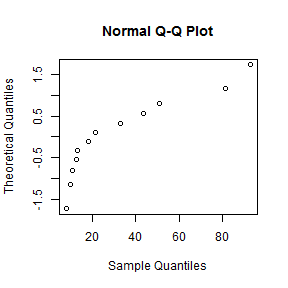
\includegraphics[width=\maxwidth]{figure/ex06-14} 

\end{knitrout}


\section{Chapter 7}



\section[Chapter 8]{Chapter 8, Confidence Intervals for One Population Mean}

\subsection{Example 8.1, Estimating a Population Mean}
\begin{knitrout}
\definecolor{shadecolor}{rgb}{0.969, 0.969, 0.969}\color{fgcolor}\begin{kframe}
\begin{alltt}
\hlcom{#read in the data}
\hlstd{prices} \hlkwb{<-} \hlkwd{read.csv}\hlstd{(}\hlstr{"data/Tb08-01.txt"}\hlstd{)}
\hlkwd{str}\hlstd{(prices)}
\end{alltt}
\begin{verbatim}
## 'data.frame':	36 obs. of  1 variable:
##  $ PRICE: num  53.8 54.4 45.2 42.9 49.9 48.2 41.6 58.9 48.6 53.1 ...
\end{verbatim}
\begin{alltt}
\hlkwd{hist}\hlstd{(prices}\hlopt{$}\hlstd{PRICE,} \hlkwc{breaks} \hlstd{=} \hlnum{5}\hlstd{)}
\end{alltt}
\end{kframe}
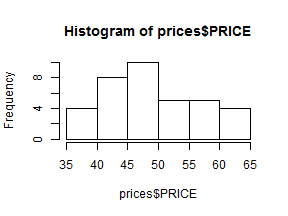
\includegraphics[width=\maxwidth]{figure/ex08-01} 
\begin{kframe}\begin{alltt}
\hlstd{sum} \hlkwb{<-} \hlkwd{sum}\hlstd{(prices}\hlopt{$}\hlstd{PRICE)}
\hlstd{n} \hlkwb{<-} \hlkwd{nrow}\hlstd{(prices)}
\hlstd{mu} \hlkwb{<-} \hlstd{sum} \hlopt{/} \hlstd{n}
\hlcom{#alternatively}
\hlstd{mu1} \hlkwb{<-} \hlkwd{mean}\hlstd{(prices}\hlopt{$}\hlstd{PRICE)}
\end{alltt}
\end{kframe}
\end{knitrout}

\paragraph{}The estimated population, $\mu$, from the sample mean, $\bar{x}$, is 49.2778.

\subsection{Example 8.2, Introducing Confidence Intervals}
\begin{knitrout}
\definecolor{shadecolor}{rgb}{0.969, 0.969, 0.969}\color{fgcolor}\begin{kframe}
\begin{alltt}
\hlcom{#read in the data}
\hlstd{prices} \hlkwb{<-} \hlkwd{read.csv}\hlstd{(}\hlstr{"data/Tb08-01.txt"}\hlstd{)}
\hlkwd{str}\hlstd{(prices)}
\end{alltt}
\begin{verbatim}
## 'data.frame':	36 obs. of  1 variable:
##  $ PRICE: num  53.8 54.4 45.2 42.9 49.9 48.2 41.6 58.9 48.6 53.1 ...
\end{verbatim}
\begin{alltt}
\hlkwd{hist}\hlstd{(prices}\hlopt{$}\hlstd{PRICE,} \hlkwc{breaks} \hlstd{=} \hlnum{5}\hlstd{)}
\end{alltt}
\end{kframe}
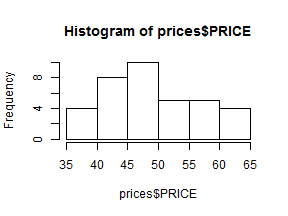
\includegraphics[width=\maxwidth]{figure/ex08-02} 
\begin{kframe}\begin{alltt}
\hlstd{sum} \hlkwb{<-} \hlkwd{sum}\hlstd{(prices}\hlopt{$}\hlstd{PRICE)}
\hlstd{n} \hlkwb{<-} \hlkwd{nrow}\hlstd{(prices)}
\hlstd{mu} \hlkwb{<-} \hlstd{sum} \hlopt{/} \hlstd{n}
\hlstd{sigma} \hlkwb{<-} \hlnum{7.2}
\hlstd{s} \hlkwb{<-} \hlstd{sigma} \hlopt{/} \hlkwd{sqrt}\hlstd{(n)}
\hlkwd{cat}\hlstd{(sum, n, mu, sigma, s)}
\end{alltt}
\begin{verbatim}
## 1774 36 49.28 7.2 1.2
\end{verbatim}
\begin{alltt}
\hlstd{confidence.interval} \hlkwb{<-} \hlkwd{simple.z.test}\hlstd{(prices}\hlopt{$}\hlstd{PRICE, sigma,} \hlkwc{conf.level} \hlstd{=} \hlnum{0.9544}\hlstd{)}
\hlstd{confidence.interval}
\end{alltt}
\begin{verbatim}
## [1] 46.88 51.68
\end{verbatim}
\end{kframe}
\end{knitrout}

\subsection{Example 8.3, Interpreting Confidence Intervals}

\subsection{Example 8.1, }


\section[Chapter 9]{Chapter 9, Hypothesis Tests for One Population Mean}

\subsection{Example 9.1, Choosing the Null and Alternative Hypotheses}This example contains no code.
\subsection{Example 9.2, Choosing the Null and Alternative Hypotheses}This example contains no code.
\subsection{Example 9.3, Choosing the Null and Alternative Hypotheses}This example contains no code.
\subsection{Example 9.4, The Logic of Hypothesis Testing}

Null hypothesis is $H_0: \mu = 454$. \\
Alternative hypothesis is $H_\alpha: \mu \not= 454$.

\begin{knitrout}
\definecolor{shadecolor}{rgb}{0.969, 0.969, 0.969}\color{fgcolor}\begin{kframe}
\begin{alltt}
\hlcom{# load the data file}
\hlstd{weights} \hlkwb{<-} \hlkwd{read.csv}\hlstd{(}\hlstr{"data/Tb09-01.txt"}\hlstd{)}
\hlkwd{str}\hlstd{(weights)}
\end{alltt}
\begin{verbatim}
## 'data.frame':	25 obs. of  1 variable:
##  $ WEIGHT: int  465 456 438 454 447 449 442 449 446 447 ...
\end{verbatim}
\begin{alltt}
\hlcom{#declare and initialize variables}
\hlstd{mu} \hlkwb{<-} \hlnum{454}
\hlstd{sigma} \hlkwb{<-} \hlnum{7.8}
\hlstd{n} \hlkwb{<-} \hlnum{25}
\hlstd{xbar} \hlkwb{<-} \hlkwd{mean}\hlstd{(weights}\hlopt{$}\hlstd{WEIGHT)}
\hlstd{ztest} \hlkwb{<-} \hlstd{(xbar} \hlopt{-} \hlstd{mu)} \hlopt{/} \hlstd{(sigma} \hlopt{/} \hlkwd{sqrt}\hlstd{(n))}
\hlstd{ztest}
\end{alltt}
\begin{verbatim}
## [1] -2.564
\end{verbatim}
\begin{alltt}
\hlcom{#determine the result of the test}
\hlstd{result} \hlkwb{<-} \hlkwd{pnorm}\hlstd{(ztest)}
\hlstd{result}
\end{alltt}
\begin{verbatim}
## [1] 0.005172
\end{verbatim}
\begin{alltt}
\hlcom{#use simple z test from UsingR package}
\hlkwd{library}\hlstd{(UsingR)}
\hlstd{conf.int} \hlkwb{<-} \hlkwd{simple.z.test}\hlstd{(weights}\hlopt{$}\hlstd{WEIGHT,} \hlkwc{sigma} \hlstd{= sigma,} \hlkwc{conf.level} \hlstd{=} \hlnum{0.9544}\hlstd{)}
\hlstd{conf.int}
\end{alltt}
\begin{verbatim}
## [1] 446.9 453.1
\end{verbatim}
\end{kframe}
\end{knitrout}

\paragraph{}The claimed weight of the population is $\mu{}$ per bag, $454$ grams. The mean sample weight is $\bar{x}$ per bag, $450$ grams. The $z$ value is $\ensuremath{-2.5641}$, which is more than two standard deviations below the population mean. 


\subsection{Example 9.5, Type I and Type II Errors}This example contains no code.
\subsection{Example 9.6, Obtaining the Critical Values}

\begin{knitrout}
\definecolor{shadecolor}{rgb}{0.969, 0.969, 0.969}\color{fgcolor}\begin{kframe}
\begin{alltt}
\hlstd{left.tail} \hlkwb{<-} \hlkwd{qnorm}\hlstd{(}\hlnum{0.05}\hlstd{)}
\hlstd{left.tail}
\end{alltt}
\begin{verbatim}
## [1] -1.645
\end{verbatim}
\begin{alltt}
\hlstd{right.tail} \hlkwb{<-} \hlkwd{qnorm}\hlstd{(}\hlnum{0.95}\hlstd{)}
\hlstd{right.tail}
\end{alltt}
\begin{verbatim}
## [1] 1.645
\end{verbatim}
\begin{alltt}
\hlstd{two.tail.left} \hlkwb{<-} \hlkwd{qnorm}\hlstd{(}\hlnum{0.025}\hlstd{)}
\hlstd{two.tail.left}
\end{alltt}
\begin{verbatim}
## [1] -1.96
\end{verbatim}
\begin{alltt}
\hlstd{two.tail.right} \hlkwb{<-} \hlkwd{qnorm}\hlstd{(}\hlnum{0.975}\hlstd{)}
\hlstd{two.tail.right}
\end{alltt}
\begin{verbatim}
## [1] 1.96
\end{verbatim}
\end{kframe}
\end{knitrout}

\subsection{Example 9.7, The One-Sample z-Test}

Null hypothesis is $H_0: \mu = \$51.46$. \\
Alternative hypothesis is $H_\alpha: > \$51.46$

\begin{knitrout}
\definecolor{shadecolor}{rgb}{0.969, 0.969, 0.969}\color{fgcolor}\begin{kframe}
\begin{alltt}
\hlcom{# load the data file}
\hlstd{books} \hlkwb{<-} \hlkwd{read.csv}\hlstd{(}\hlstr{"data/Tb09-05.txt"}\hlstd{)}
\hlkwd{str}\hlstd{(books)}
\end{alltt}
\begin{verbatim}
## 'data.frame':	40 obs. of  1 variable:
##  $ PRICE: num  56 46.2 47.3 54 53.7 ...
\end{verbatim}
\begin{alltt}
\hlcom{#declare and initialize variables}
\hlstd{mu} \hlkwb{<-} \hlnum{51.46}
\hlstd{sigma} \hlkwb{<-} \hlnum{7.61}
\hlstd{n} \hlkwb{<-} \hlnum{40}
\hlstd{xbar} \hlkwb{<-} \hlkwd{mean}\hlstd{(books}\hlopt{$}\hlstd{PRICE)}
\hlstd{right.tail} \hlkwb{=} \hlnum{0.01}
\hlstd{ztest} \hlkwb{<-} \hlstd{(xbar} \hlopt{-} \hlstd{mu)} \hlopt{/} \hlstd{(sigma} \hlopt{/} \hlkwd{sqrt}\hlstd{(n))}
\hlstd{ztest}
\end{alltt}
\begin{verbatim}
## [1] 2.851
\end{verbatim}
\begin{alltt}
\hlstd{right.crit} \hlkwb{<-} \hlkwd{qnorm}\hlstd{(}\hlnum{1} \hlopt{-} \hlstd{right.tail)}
\hlstd{right.crit}
\end{alltt}
\begin{verbatim}
## [1] 2.326
\end{verbatim}
\end{kframe}
\end{knitrout}

\paragraph{}The $z$ statistic is 2.8508, which is greater than the critical value of 2.3263, so we reject the null hypothesis.

\subsection{Example 9.8, The One-Sample z-Test}

Null hypothesis is $H_0: \mu = 800$. \\
Alternative hypothesis is $H_\alpha: < 800$

\begin{knitrout}
\definecolor{shadecolor}{rgb}{0.969, 0.969, 0.969}\color{fgcolor}\begin{kframe}
\begin{alltt}
\hlcom{# load the data file}
\hlstd{rda} \hlkwb{<-} \hlkwd{read.csv}\hlstd{(}\hlstr{"data/Tb09-06.txt"}\hlstd{)}
\hlkwd{str}\hlstd{(rda)}
\end{alltt}
\begin{verbatim}
## 'data.frame':	18 obs. of  1 variable:
##  $ CALCI: int  686 433 743 647 734 641 993 620 574 634 ...
\end{verbatim}
\begin{alltt}
\hlcom{#declare and initialize variables}
\hlstd{mu} \hlkwb{<-} \hlnum{800}
\hlstd{sigma} \hlkwb{<-} \hlnum{188}
\hlstd{n} \hlkwb{<-} \hlnum{18}
\hlstd{xbar} \hlkwb{<-} \hlkwd{mean}\hlstd{(rda}\hlopt{$}\hlstd{CALCI)}
\hlstd{left.tail} \hlkwb{=} \hlnum{0.05}
\hlstd{ztest} \hlkwb{<-} \hlstd{(xbar} \hlopt{-} \hlstd{mu)} \hlopt{/} \hlstd{(sigma} \hlopt{/} \hlkwd{sqrt}\hlstd{(n))}
\hlstd{ztest}
\end{alltt}
\begin{verbatim}
## [1] -1.187
\end{verbatim}
\begin{alltt}
\hlstd{left.crit} \hlkwb{<-} \hlkwd{qnorm}\hlstd{(left.tail)}
\hlstd{left.crit}
\end{alltt}
\begin{verbatim}
## [1] -1.645
\end{verbatim}
\end{kframe}
\end{knitrout}

\paragraph{}The $z$ statistic is \ensuremath{-1.1873}, which is less than the critical value of \ensuremath{-1.6449}, so we do not reject the null hypothesis.

\subsection{Example 9.9, The One-Sample z-Test}

Null hypothesis is $H_0: \mu = 60$. \\
Alternative hypothesis is $H_\alpha: \not= 60$

\begin{knitrout}
\definecolor{shadecolor}{rgb}{0.969, 0.969, 0.969}\color{fgcolor}\begin{kframe}
\begin{alltt}
\hlcom{# load the data file}
\hlstd{cheetah} \hlkwb{<-} \hlkwd{read.csv}\hlstd{(}\hlstr{"data/Tb09-07.txt"}\hlstd{)}
\hlkwd{str}\hlstd{(cheetah)}
\end{alltt}
\begin{verbatim}
## 'data.frame':	35 obs. of  1 variable:
##  $ SPEEDS: num  57.3 57.5 59 56.5 61.3 57.6 59.2 65 60.1 59.7 ...
\end{verbatim}
\begin{alltt}
\hlcom{#histogram of the data set}
\hlkwd{hist}\hlstd{(cheetah}\hlopt{$}\hlstd{SPEEDS,} \hlkwc{breaks} \hlstd{=} \hlnum{15}\hlstd{,} \hlkwc{xlab} \hlstd{=} \hlstr{"Cheetah Speeds"}\hlstd{,} \hlkwc{ylab} \hlstd{=} \hlstr{"Counts"}\hlstd{,} \hlkwc{main} \hlstd{=} \hlstr{"Histogram of Cheetah Speeds Sample"}\hlstd{)}
\end{alltt}
\end{kframe}
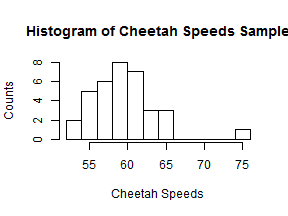
\includegraphics[width=\maxwidth]{figure/ex09-09} 
\begin{kframe}\begin{alltt}
\hlcom{#declare and initialize variables}
\hlstd{mu} \hlkwb{<-} \hlnum{60}
\hlstd{sigma} \hlkwb{<-} \hlnum{3.2}
\hlstd{n} \hlkwb{<-} \hlnum{35}
\hlstd{xbar} \hlkwb{<-} \hlkwd{mean}\hlstd{(cheetah}\hlopt{$}\hlstd{SPEEDS)}
\hlstd{tails} \hlkwb{=} \hlnum{0.05}
\hlstd{ztest} \hlkwb{<-} \hlstd{(xbar} \hlopt{-} \hlstd{mu)} \hlopt{/} \hlstd{(sigma} \hlopt{/} \hlkwd{sqrt}\hlstd{(n))}
\hlstd{ztest}
\end{alltt}
\begin{verbatim}
## [1] -0.8768
\end{verbatim}
\begin{alltt}
\hlstd{crits} \hlkwb{<-} \hlkwd{qnorm}\hlstd{(}\hlkwd{c}\hlstd{( tails} \hlopt{/} \hlnum{2}\hlstd{, (}\hlnum{1} \hlopt{-} \hlstd{tails} \hlopt{/} \hlnum{2}\hlstd{)))}
\hlstd{crits}
\end{alltt}
\begin{verbatim}
## [1] -1.96  1.96
\end{verbatim}
\end{kframe}
\end{knitrout}

\paragraph{}The $z$ statistic is \ensuremath{-0.8768}, which is less than the critical values of \ensuremath{-1.96}, 1.96, so we do not reject the null hypothesis.

\subsection{Example 9.10, }
\subsection{Example 9.11, }
\subsection{Example 9.12, }
\subsection{Example 9.13, }
\subsection{Example 9.14, }
\subsection{Example 9.15, }
\subsection{Example 9.16, }
\subsection{Example 9.17, }
\subsection{Example 9.18, }
\subsection{Example 9.19, }
\subsection{Example 9.20, }
\subsection{Example 9.21, }

\section{Chapter 10}


\section{Chapter 11}



\end{document}
